\section{Preliminaries} \label{sec:prelim}

\subsection{Rasmussen's construction}

We review the definition of the reduced HOMFLY homology, following Rasmussen \cite{Ras15}.
% 
Let $D$ be an oriented link diagram, and $G(D)$ the underlying projection
% , which can be
regarded as an oriented $4$-valent graph.
For simplicity, we assume that $D$ is non-trivial (i.e.\ has at least one crossing) and that $D$ is connected (i.e.\ $G(D)$ is connected).

First we define the \textit{reduced edge ring} $R(D)$ of $D$.
Associate an indeterminate $x_e$ to each edge $e$ of $G(D)$, and let $R'(D)$ be the multivariate polynomial ring $\QQ[x_e]$ generated by them.
Endow a $\ZZ$-grading on $R'(D)$, called the \textit{$q$-grading}, by declaring that every generator $x_e$ has degree $2$.
% 
Define $\theta = \sum_e x_e \in R'(D) $, and for each crossing $p$ of $D$,
\[
    \rho_p = x_a+x_b-x_c-x_d \in R'(D),
\]
where $a, b$ are outgoing edges at $p$ and $c,d$ are incoming edges at $p$ (see \Cref{complex}).
Let $I(D)$ be the ideal of $R'(D)$ generated by $\theta$ and $\rho_{p}$ for all crossings $p$ in $D$.
$R(D)$ is defined by the quotient ring $R'(D)/I(D)$.
Since $I(D)$ is a homogeneous ideal, the $q$-grading on  $R'(D)$ is inherited to $R(D)$.

\begin{remark}
    Since we only deal with the reduced theory, we simply write $R(D)$ instead of $R_r(D)$ as written in \cite{Ras15}.
\end{remark}

Next 
%, for the diagram $D$, 
we define a double chain complex $C(D)$ over $R = R(D)$. We start with some conventions and terminologies.
The complex $C(D)$ has two homological gradings, called the \textit{horizontal grading} and the \textit{vertical grading}.
It also has an internal grading, again called the \textit{$q$-grading}, which is compatible with the grading on $R$.
%(We note that it is not compatible with one of the differentials.)
We denote by $C^{*,j,k}(D)$ the $R$-module in $C(D)$ on horizontal degree $j$ and vertical degree $k$, and by $C^{i,j,k}(D)$ the homogeneous $\QQ$-subspace of $C(D)$ with $q$-degree $i$ in $C^{*,j,k}(D)$.

There are two differentials $d_H, d_V$ on $C(D)$, which are called the \textit{horizontal differential} and the \textit{vertical differential} respectively. The differentials $d_H, d_V$ are homogeneous with triple degrees $(2,2,0)$ and $(0,0,2)$, respectively. The complex $C^{*,j,k}(D)$ will be supported on even $j,k$.

The construction of $C(D)$ follows.
For a crossing $p$ in $D$, we define a double complex $C_p(D)$ by the diagrams in \Cref{complex}, depending on the sign of $p$.
In the figure, the horizontal arrows indicate $d_H$ and the vertical arrows indicate $d_V$.
Each arrow is labeled by 
% an element $x$ in $R$, which indicates the multiplication map by $x$.
a polynomial $f \in R$, which indicates that the map is given by the multiplication by $f$. 
The subscripts $a,b,c,d$ indicates the edges around $p$, as shown on the right of the figure.
The notation $R\{i,j,k\}$ indicates a copy of $R$ on homological bidegree $(j,k)$ with $q$-grading shifted so that $1 \in R$ has $q$-degree $i$.

\begin{figure}[t]
\begin{center}
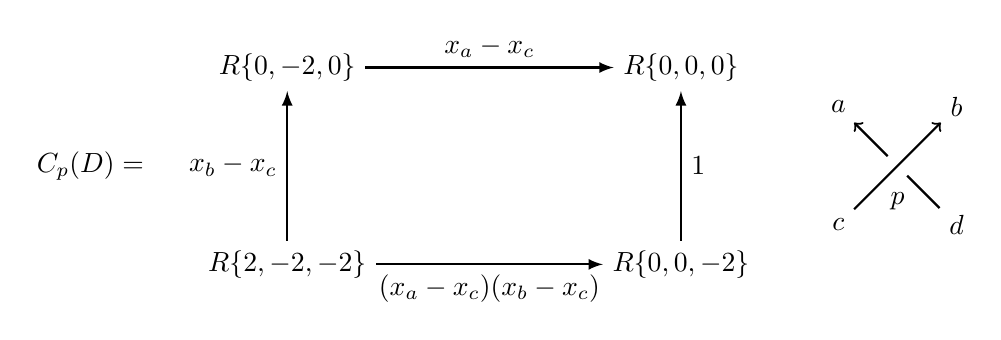
\begin{tikzpicture}[auto]
    \node (a) at (0, 0) {$R\{2,-2,-2\}$};
    \node (b) at (0,2.5) {$R\{0,-2,0\}$};
    \node (c) at (5,0) {$R\{0,0,-2\}$};
    \node (d) at (5,2.5) {$R\{0,0,0\}$};
    \node (C) at (-2.5, 1.25) {$C_p(D)=$};
    \draw[-latex, thick] (a) to node {$x_b-x_c$} (b);
    \draw[-latex, thick] (a) to node[swap] {$ (x_a-x_c)(x_b-x_c)$} (c);
    \draw[-latex, thick] (b) to node {$x_a-x_c$} (d);
    \draw[-latex, thick] (c) to node[swap] {$1$} (d);
    \node (p) at (7.75, 0.8) {$p$};
    \node (v1) at (7,2) {$a$};
    \node (v2) at (8.5,2) {$b$};
    \node (v3) at (7,0.5) {$c$};
    \node (v4) at (8.5,0.5) {$d$};
    \node (center) at (7.75,1.25) {};
    \draw [->, thick] (v3) edge (v2);
    \draw [->, thick] (center) edge (v1);
    \draw [thick] (v4) edge (center);
\end{tikzpicture}

\vspace{12pt}
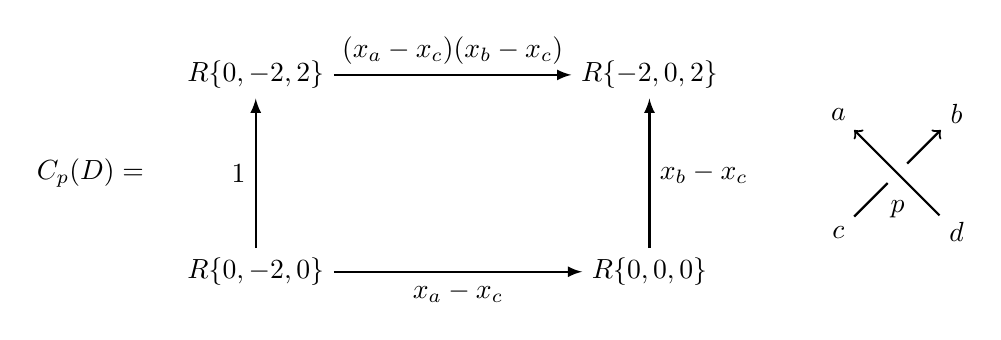
\begin{tikzpicture}[auto]
    \node (a) at (-0.4, 0) {$R\{0,-2,0\}$};
    \node (b) at (-0.4,2.5) {$R\{0,-2,2\}$};
    \node (c) at (4.6,0) {$R\{0,0,0\}$};
    \node (d) at (4.6,2.5) {$R\{-2,0,2\}$};
    \node (C) at (-2.5, 1.25) {$C_p(D)=$};
    \draw[-latex, thick] (a) to node {$1$} (b);
    \draw[-latex, thick] (a) to node[swap] {$x_a-x_c$} (c);
    \draw[-latex, thick] (b) to node {$ (x_a-x_c)(x_b-x_c)$} (d);
    \draw[-latex, thick] (c) to node[swap] {$x_b-x_c$} (d);
    \node (p) at (7.75, 0.8) {$p$};
    \node (v1) at (7,2) {$a$};
    \node (v2) at (8.5,2) {$b$};
    \node (v3) at (7,0.5) {$c$};
    \node (v4) at (8.5,0.5) {$d$};
    \node (center) at (7.75,1.25) {};
    \draw [->, thick] (v4) edge (v1);
    \draw [->, thick] (center) edge (v2);
    \draw [thick] (v3) edge (center);
\end{tikzpicture}
\end{center}
\caption{The definition of $C_p(D)$}\label{complex}
\end{figure}

We immediately see that $d_H$ and $d_V$ commute in $C_p(D)$ and that the triple degrees of $d_H$ and $d_V$ are indeed $(2,2,0)$ and $(0,0,2)$, respectively.  
Define $C(D)$ as the tensor product (over $R$) of $C_p(D)$ taken among all crossings $p$ of $D$.

Now define the (\textit{unshifted}) \textit{homology}
\[
    \Hhat(D) = H(H(C(D), d_H), (d_V)_*).
\]
This reads: first take the homology of $C(D)$ by the horizontal differential $d_H$, and then take homology of $H(C(D), d_H)$ by the induced differential $(d_V)_*$. 

\begin{definition}
    Let $w$ be the writhe of $D$, and let $s$ be the number of Seifert circles of $D$.
    The homology $\Hbar(D)$ of $D$ is given by
    \begin{equation} \label{eq:Hbar-def}
        \Hbar(D) = \Hhat(D)\{-w+s-1,w+s-1,w-s+1\},
    \end{equation}
    where here the notation $\{i, j, k\}$ indicates a shift of triple gradings.
\end{definition}

\begin{theorem}[\cite{KR08, Ras15}]
    Let $L$ be a link. The isomorphism class of $\Hbar(D)$ as a triply graded vector space is independent of the choice of $D$, provided that $D$ is a closed braid diagram of $L$.
\end{theorem}

\begin{definition}
    For a link $L$, 
    we denote by $\Hbar(L)$ the homology group $\Hbar(D)$ for a closed braid diagram $D$ of $L$, and call it the \textit{reduced HOMFLY homology} of $L$.
\end{definition}

\begin{remark}\label{rem:generaldiag}
    Unless $D$ is a closed braid diagram of $L$, the homology $\Hbar(D)$ generally does \textit{not} give the HOMFLY homology $\Hbar(L)$.
    Further considerations are given in \Cref{sec:future}. 
\end{remark}

\begin{definition}
    The Poincar\'e series of $\Hbar(L)$ is denoted by
    \[
        \mathcal{P}(L) = \sum_{i,j,k} q^ia^jt^{(k-j)/2}\dim \Hbar^{i,\,j,\,k}(L).
    \]
\end{definition}

The following theorem states that the graded Euler characteristic of the HOMFLY homology $\Hbar(L)$ gives the HOMFLY polynomial $P(L)$. 

\begin{theorem}[\cite{KR08, Ras15}]
    For any oriented link $L$, we have
    \begin{equation*}
        P(L)(q,a) = \mathcal{P}(L)(q,a,-1).  
    \end{equation*}
\end{theorem}

\subsection{MFW bounds and dualities}

We recall several important results on the reduced HOMFLY homology of knots, which are essential in proving the finiteness of our algorithm.

The following is a categorified version of the \textit{Morton-Franks-Williams Inequality} \cite{Mor86, FW87}.
%
\begin{proposition}[{\cite{Kho07, Wu08}}] \label{prop:MFW-ineq}
    For a link $L$ with braid closure diagram $D$, the HOMFLY homology $\Hbar^{*, j, *}(L)$ is supported in
    \[
        j \in [w - s + 1,\ w + s - 1],
    \]
    where $w, s$ denote the writhe and the number of Seifert circles of $D$ respectively. 
\end{proposition}

The following is a categorified version of the symmetry of the HOMFLY polynomial $P_K(q,a) = P_K(-q^{-1}, a)$, which had been conjectured since the foundation of HOMFLY homology theory.

\begin{proposition}[{\cite{DGR,OR20,gorsky2021:tautological}}] \label{prop:q-sym}
    For a knot $K$,
    \[
        \Hbar^{i, j, k}(K) \isom \Hbar^{-i, j, k + 2i}(K).
    \]
\end{proposition}

From this, we obtain a categorified version of the \textit{Morton bound} \cite{Mor86}.

\begin{proposition} \label{prop:morton}
    For a knot $K$ with braid closure diagram $D$, $\Hbar^{i, *, *}(K)$ is supported in
    \[
        i \in [-n + s - 1,\ n - s + 1],
    \]
    where $n, s$ denote the number of crossings and the number of Seifert circles of $D$ respectively. 
\end{proposition}

\begin{proof}
    Let $n^-$ be the number of negative crossings of $D$. From \Cref{complex}, it is obvious that the lowest $q$-degree with non-trivial chain group in $C(D)$ is $-2n^-$. The corresponding shifted degree in $\Hbar(D)$ gives the lower bound. The upper bound follows from the symmetry.
\end{proof}

Finally, the following is the duality on mirrors of knots.

\begin{proposition}[\cite{EMAK}] \label{prop:duality}
    For a knot $K$ and its mirror $m(K)$,
    \[
        \Hbar^{i, j, k}(m(K)) \isom \Hbar^{-i, -j, -k}(K).
    \]
\end{proposition}

\begin{proof}
    One can use the K\"unneth universal coefficient spectral sequence to deduce this isomorphism from the duality given in Corollary 1.12 of \cite{EMAK}.
    The spectral sequence converges at the $E_2$ page, since any variable in the reduced base polynomial ring acts as zero on the homology $\Hbar(K)$ of a knot $K$ (which is an analogous fact of \cite[Lemma 5.16]{Ras15}).
\end{proof}